\documentclass[submission]{iacrtrans}

\usepackage[T1]{fontenc}
\usepackage[
    backend=biber,
    style=numeric,
    natbib=true,
    url=false, 
    doi=true,
    eprint=false
    ]{biblatex}
\addbibresource{paper.bib}
\usepackage{amssymb,amsmath}
\usepackage{eurosym}
\usepackage{wasysym}
\usepackage[binary-units]{siunitx}
\usepackage{commath}
\usepackage{graphicx,color}
\usepackage{colortbl}
\usepackage{subcaption}
\usepackage{placeins}
\usepackage{array}
\usepackage{censor}
\usepackage{hyperref}
\usepackage{makecell}

\DeclareSIUnit{\baud}{Bd}
\DeclareSIUnit{\year}{a}
\DeclareSIUnit{\rpm}{rpm}
\renewcommand{\floatpagefraction}{.8}
\newcommand{\degree}{\ensuremath{^\circ}}
\newcolumntype{P}[1]{>{\centering\arraybackslash}p{#1}}
\newcommand{\partnum}[1]{\texttt{#1}}
\newcommand{\todo}[1]{\textbf{TODO}\footnote{#1}}
% Set to 1.0 for final two-column export
\newlength{\figurescale}
\setlength{\figurescale}{0.75\textwidth}

\begin{document}

\author{Jan Sebastian Götte\inst{1} \and Björn Scheuermann\inst{2}}
\institute{Technical University of Darmstadt, Darmstadt, Germany, \email{jan.goette@tu-darmstadt.de}\and
    Technical University of Darmstadt, Darmstadt, Germany, \email{bjoern.scheuermann@kom.tu-darmstadt.de}}
\title{High Fidelity Security Mesh Monitoring using Low-Cost, Embedded Time Domain Reflectometry}
\maketitle

% FIXME maybe don't use HSM, maybe use active tamper sensing? envelope protection?

\begin{abstract}
    Security Meshes are patterns of sensing traces covering an area that are used in Hardware Security Modules (HSMs) to
    detect attempts at physical intrusion into the HSM's protective shell. In this paper, we present an optimized,
    embeddable security mesh monitoring circuit that applies the principles behind Time Domain Reflectometry (TDR) to
    create a unique fingerprint of a mesh, and to detect not only DC faults, but also attempts at bridging and removing
    parts of the mesh. Our TDR circuit improves over previous low-cost TDR approaches by utilizing exclusively low-cost,
    consumer-grade components with a total Bill of Materials (BoM) cost of less than 10\$ while achieving a time
    resolution better than \qty{200}{\pico\second}.
    % We validate our mesh monitoring system in a number of realistic attack scenarios using a real-time, embeddable
    % Machine Learning (ML) classifier.
    % TODO: Use Dynamic Time Warping to compare traces?
\end{abstract}

\todo{In abstract: specific bandwidth / risetime numbers.}
\todo{In abstract: Add machine learning / "AI" classifier.}

\section{Introduction}

Security meshes continue to be the state of the art for tamper sensing in in applications where sophisticated physical
attacks must be prevented. Security meshes usually consist of two or more conductive traces that are laid out in a
meandering pattern to cover a surface, and which are monitored electrically to detect attempts at penetrating this
surface. Security meshes can be implemented at the macro scale, covering entire Printed Circuit Board Assemblies
(PCBAs) in applications such as Hardware Security Modules (HSMs) or card payment terminals, or they can be implemented
at the micro scale to prevent the readout of secrets from Integrated Circuits (ICs) such as smartcards or Trusted
Platform Modules (TPMs). Micro-scale tamper sensing meshes are usually as passive sensors without a continuous power
supply, and are only checked once during system powerup, macro-scale meshes are usually implemented as active sensors
with a continuous backup power supply so as to not give the attacker a window of attack when the remaining system is
powered down.

There are some academic works suggesting the use of security meshes as Physically Uncloneable Functions (PUFs) to
provide a high-fidelity tamper sensor that can even detect attempts at patching the mesh to fix traces broken in a
drilling attack. While early work in this area was limited in the size of the protected envelope, recent advancements
allow for the protection of entire PCBAs similar in size to common commercial systems such as HSMs or the processing
subsystems of card payment terminals.

As is often the case with security technologies, in practice there exists a tension between the level of security
offered by a particular security mesh implementation, and its implementation cost. The most secure meshes require
specialized manufacturing techniques that aim to produce what is essentially a Flexible Printed Circuit (FPC) whose
materials are specifically chosen to be as fragile as possible such that it breaks even during careful manipulation by
an attacker.

In contrast to this in the industry, simpler approaches are still commonly used for their ease of implementation. Often,
standard copper/polyimide FPCs are used because of the wide availability of manufacturing services. In some
lower-security applications such as card payment terminals, meshes manufactured from simple PCBs are even used to
provide protection in directions considered especially vulnerable, without enclosing the whole PCBA.

In this paper, we introduce an approach for the design of security mesh monitoring circuitry that provides dramatically
higher fidelity compared to state-of-the-art conductivity monitoring, improving the sensitivity of meshes even when
manufactured using less advanced technologies such as standard FPC or PCB processes. Our approach consists of an
optimized, low-cost differential Time Domain Reflectometry (TDR) frontend that provides better than
\qty{200}{\pico\second}( resolution, connected to a security mesh. Using our TDR frontend, mesh integrity can be
characterized at high fidelity, producing several hundred measurements for each meter of mesh trace length.


\todo{citations for applications}

%HSMs predate modern cryptography.
%\cite{nsaHistoryUSCommunications1973, nsaHistoryUSCommunications1981}

\section{Related Work}

% cite satoToucheEnhancingTouch2012 on capacitive fingerprinting

While security meshes are widely used in practice, their design is only covered by a sparse research corpus.

% TODO more citations to their papers here
\paragraph{Meshes as capacitive PUFs}
The most advanced mesh designs such as \textcite{obermaierMeasurementSystemCapacitive2018} use a specialized security
mesh as a Physically Uncloneable Function (PUF), combining tamper sensing with cryptographic key storage. In their
design, the mesh consists of a cross-hatch pattern made up from several dozen individually adressable capacitive
electrodes. Their analog frontend measures the precise mutual capacitance of each pair of electrodes, and they use the
resulting capacitance matrix as the basis of their PUF.

Advantages of their system include very high sensitivity, and that as a PUF, the system does not require a continuous
power supply. Disadvantages include limited mesh surface area and resulting small volume, the specialized and thus
costly mesh manufacturing process, and a cost-intensive monitoring circuit.

\paragraph{Bridge measurement of capacitive interdigital meshes}

\textcite{dupontMiniaturizedUltraLowPowerTamper2022} introduce a simple analog circuit approach for monitoring meshes
laid out as a set of capacitive interdigital structures not unlike the combs found in Micro-Electromechanical System
(MEMS) accelerometers and gyroscopes. They subdivide the mesh into four equal-sized quadrants, each containing two
equal-size interdigital electrodes. They connect the resulting eight electrodes in a capacitive bridge configuration,
and measure the bridge's balance using a simple analog monitoring circuit.

Advantages of their system include the simple, low power monitoring circuit made up from basic, cheap components and the
capability to work with single-layer meshes such as those produced using Laser Direct Structuring (LDS).

\paragraph{Frequency-domain mesh characterization}
\textcite{vasileProtectingSecretsAdvanced2019} introduce a monitoring method where they feed a variable-frequency signal
into one end of a continuous mesh trace, and measure the power of the signal coming out of the other end. In essence,
their setup measures $S_{12}$ magnitude in a similar way to a network analyzer.

Advantages of their design include the simple implementation, and the potentially robust nature of frequency-domain
measurements. Disadvantages include a nonstandard three-layer mesh stackup, as well as the susceptibility of the system
to attack by emulation given that the log power sensor they are using at the mesh output is designed to be insensitive
to any signal characteristics apart from total signal power.

\paragraph{Time-domain mesh monitoring}
\textcite{vasileActiveTamperDetection2017,vasileTemperatureSensitiveActive2017} propose monitoring the time-domain
response of a mesh using a circuit made up from a pulse generator and a fast analog-to-digital converter (ADC). To avoid
the need for a full high-speed data processing pipeline, their design is centered around a specialized high-speed ADC
that has a small built-in sample memory, allowing them to capture a pulse at high speed before slowly processing it from
sample memory.

Advantages of their design include better sensitivity to changes in total mesh trace length compared to simple
continuity monitoring and the low complexity of their analog frontend. Disadvantages include the high cost of the
specialized components, coarse time resolution of \qty{5}{\nano\second} and the choice of a $S_{12}$ measurement
configuration, which while sensitive to changes in \emph{length}, is insensitive to changes in \emph{impedance}. In
contrast, a TDR approach measuring $S_11$ when used with a reflector at the far end of the mesh will detect both changes
in overall length and changes in impedance.

\subsection{Security Mesh Monitoring and Design}

\cite{vasileTemperatureSensitiveActive2017}
\cite{vasileActiveTamperDetection2017}

\subsection{Hardware Security Module System Design}

\cite{dupontMiniaturizedUltraLowPowerTamper2022}

\subsection{Equivalent-Time Sampling}

Today, systems that digitize high-speed signals usually use a fast ADC, sometimes preceded by one or several
downconverting mixers. This development was enabled by both the increasing availability of ADCs capable of digitizing
hundreds of megasamples per second at a reasonable resolution, and by the increase in speed and capability of CPUs,
FPGAs and other digital components enabling the processing of the large amounts of data generated by such converters in
real time. However, this is largely a development of this millennium--meanwhile, signals far into the gigahertz range
have been studied since the advent of radar technology in the second world war\cite{kahrs50YearsRF2003}. Enabled by the
progress from vacuum tubes to semiconductor devices, equivalent-time sampling became the technology of choice for the
latter half of the twentieth century until around the turn of the millenium the introduction of high-speed digital
processing and fast ADCs enabled real-time conversion up into higher microwave frequencies, reaching beyond the
\qty{100}{\giga\hertz} boundary these days.

\textcite{kahrs50YearsRF2003} trace back the style of four-diode balanced bridge sampling gate that we use to a vacuum
tube implementation presented in \textcite{chanceWaveforms1949}. This style of sampling gate found application in a
number of sampling oscilloscopes throughout the twentieth century in a number of oscilloscope sampling frontends such as
HP's 187B\cite{HP187BDualTrace1962}. 

While initially equivalent-time sampling was used to circumvent technological limitations, more recently it has also
been used to achieve cost-optimized designs. An example of this is \todo{cite magazine article referenced at
http://www.redrok.com/sampscope.htm -> ULB}, published in \todo{year}, which presents an external sampling frontend to
extend the capabilities of then affordable $\approx\qty{10}{\mega\hertz}$ oscilloscopes to a bandwidth of
\qty{1}{\giga\hertz}.

Going along similar principles, \todo{cite \url{https://github.com/MR-DOS/TDR_diploma_thesis/tree/master}} presents a
design for a minimal sampling TDR circuit that uses a CMOS clock generator IC along with a CML fanout buffer for pulse
generation. The circuit uses the same double sampling topology also used by \todo{cite previous source, magazine
article} to reconstruct a downsampled copy of the input signal in the analog domain before digitization.

\todo{bencivenniTimeDomainReflectometer2013}
\todo{negreaSequentialSamplingTime2009}
\todo{lee16psresolutionRandomEquivalent2003}
\todo{MiniaturizedFPGABasedHighResolution}

\subsection{Low-Cost Time Domain Reflectometry}

\subsection{Machine Learning and Anomaly Detection}

\section{Time-Domain Reflectometry}

An issue with a plain TDR measurement is that it only measures reflected signal components. If we connected a TDR
frontend to one end of a security mesh, then placed termination matched to the mesh's characteristic impedance at the
far end of the mesh, in an intact mesh that has constant impedance along its length, our TDR would measure nothing. The
transmitted pulse would simply tranverse the mesh, and be absorbed entirely by the termination. In this scenario, an
attacker could cut the mesh at any point along its length by simply placing matched termination there.

The obvious solution to this issue would be to measure not just the reflected signal component, but also its transmitted
component. However, this solution would incur additional component cost and requires the far end of the mesh to return
to the TDR circuit.

A better solution to this issue is to exploit the low insertion loss of the mesh and to place an impedance discontinuity
at the far end of the mesh, resulting in most of the incident pulse being reflected back. In an intact mesh, this will
lead to a TDR return after twice the mesh's transit time. By realizing this impedance discontinuity as a short, the
reflection will have opposite sign to the incident pulse, allowing for easy detection during signal processing.

\section{Circuit Design and Driving Approach}

A TDR can be broken down into three basic components. First, we need a source of fast pulses (or fast edges!) to
stimulate the mesh. Second, we need a coupler that allows us to couple the stimulus pulses into the mesh, and their
reflections out of it. Finally, we need a fast ADC to capture the reflections.

The focus of our circuit design is on cost. Since physical attacks happen on a time scale of minutes or hours, we do not
need a fast acquisition rate. Thus, we chose an equivalent-time sampling setup instead of direct conversion, reducing
the requirements of our data acquisition and signal processing fronted from gigasamples per second to mere megasamples,
well within the range what a commodity microcontroller can handle. A challenge in equivalent-time sampling is
precisely phase-synchronizing the sampling pulse to the fundamental frequency of the input signal, which is usually
implemented by using a high-speed comparator. We can avoid this expensive component here since our TDR frontend
generates the stimulus signal itself. Thus, we only have to generate a sampling pulse at an adjustable phase to the
stimulus pulse.

Since an intact mesh has low insertion loss, the amplitude of the response of an intact mesh is large. Thus, we do not
need a high dynamic range in either the frontend amplifiers nor in the ADC, enabling the use of commodity operational
amplifiers (opamps) and the built-in ADC of a commodity microcontroller. Further, the strong signal allows us to use a
comparatively lossy \qty{-6}{\deci\bel} resistive tee instead of a directional coupler. A resistive tee does not provide
directionality, but in our case the incident pulse can never interfere with reflections at the sampling output of the
divider because of causality.

To implement a sub-nanosecond sampler, we chose a simple four-diode bridge sampling gate made from contemporary
commodity RF schottky diodes, which offer turn-on times better than \qty{100}{\pico\second} for less than 1€. The
four-diode configuration requires only two dual diode packages. In contrast to \todo{cite magazine article and that one
thesis here}, in our system, double sampling is not necessary - instead, we follow the sampling gate directly with an
amplifier feeding into the internal ADC of our microcontroller. We use an internal timer peripheral of the same
microcontroller to generate both stimulus and sample pulses, so we can easily phase-lock the internal ADC to the same
timer.

We base our circuit around a STM32G474RB microcontroller, a 5€-class commodity ARM microcontroller. Besides adequate
processing speed for its price class, this microcontroller offers two features that are critical to our design. First,
its internal ADCs are both higher resolution and faster than those of many older parts. % FIXME concrete numbers
Second, it is one of a few parts in its series that include a \emph{high-resolution timer} (HRTIM) peripheral that
provides several outputs that can be controlled with better than \qty{200}{\pico\second} resolution through per-output,
self-calibrating delay line circuitry. We use this peripheral to produce both the stimulus pulse and the
phase-adjustable sampling pulse.

While the HRTIM peripheral allows us to finely adjust the phase of its output waveform, the digital output structures of
the STM32G4 series are still limited to nanosecond-scale rise and fall times with the datasheet quoting
$t_r=t_f=\qty{1.7}{\nano\second}$ into a \qty{10}{\pico\farad} load when using the fastest GPIO output drive strength
setting and a \qty{3.3}{\volt} supply\todo{cite datasheet properly}. We work around this issue applying two circuit
tricks. First, we send its output through a fast amplifier to square up the edges to a rise time better than
\qty{500}{\pico\second}. The remaining challenge is that while we now have pulses with crisp edges, due to constraints
of the HRTIM peripheral, at more than \qty{10}{\nano\second}, these pulses are still much too wide to be useful. We
solve this issue by applying a clip line pulse forming network at the output of the amplifier similar to the one used in
\todo{some tek sampling head}--i.e.\ we connect the amplifier's output to the load in parallel with a short, terminated
transmission line stub. The length of this stub determines pulse width.

\subsection{Driver Selection}
%that was
%originally intended as a signal conditioner (\emph{redriver}) for DisplayPort applications. This amplifier squares
%, and can drive its output at up to \qty{1200}{\milli\volt} amplitude, which is plenty to turn on our schottky diode bridges

There are several types of amplifiers that can be used in our pulse shaping application. Common to all options, we
require differential outputs. In practice, for most parts this means we are looking for a part with Current Mode Logic
(CML) outputs. CML is a differential signaling standard that is widely used in high-speed logic. In CML, a current
source feeds a pair of transistors that steer current between the two outputs of the differential pair. By steering
current between the two outputs, common-mode currents are minimized which both reduces the effect of power supply
impedance at the transmitter, and reduces electromagnetic emissions from the differential pair's PCB traces.

\paragraph{Standard logic ICs.}
As a baseline, we will evaluate the \texttt{74LVC1G157} logic IC. This IC contains a single multiplexer, however, we are
not interested in the multiplexer functionality. The interesting trivia about this chip is that it also is one of the
only \texttt{74} series standard logic parts that has complimentary outputs. According to manufacturer specifications,
at a comparable \qty{20}{\pico\farad} load, 74LVC series parts have slightly faster rise and fall times compared to our
STM32 micrcontroller's digital IO pins\todo{cite
\url{https://www.renesas.com/en/document/apn/224-alvclvc-logic-characteristics-and-apps}}.

\paragraph{CML-Output Comparators.} Fast comparators with CML outputs such as Analog's \texttt{ADCMP606} are
easily-available, general purpose components and are easy to interface given their universal input topology. A
disadvantage of this path is that we would need one comparator each for the stimulus and strobe pulses, and these parts
are not cheap at \qtyrange{5}{10}{\euro} for one, or about \qty{3}{\euro} at a hundreds quantity.

\paragraph{Optical Networking Chipsets.}
Another category of CML-output drivers suitable for our application are a class of optical networking chipset ICs. While
today, the construction of optical transmitters has moved to direct bonding of optical components and driver ICs to
minimize parasitics, discrete driver ICs for some chipsets from the mid-2000s era are still available at reasonable
cost. Both the laser driver used to drive the transmitter laser diode, and the limiting amplifier used to amplify the
receiver photodiode's output can be used in our application, with the limiting amplifier part requiring less additional
circuitry in our application due to its lack of output bias control. In our evaluation below, we include
\texttt{MAX3748} limiting amplifier as a representative part from this category that is still commercially available. A
drawback of relying on a part like this is that its future availability is uncertain given the evolution of the
industry.

\paragraph{Bus Redrivers.}
The final category of amplifiers suitable for our pulse shaping needs is redrivers intended for high-speed data
interfaces such as USB 3, PCI express, HDMI or DisplayPort. All of these interfaces use CML, with differential voltage
levels usually in the order of \qty{1000}{\milli\volt}. Such redriver ICs are intended to be used to amplify the
sensitive high-speed bus signal at the edge of a PCBA, either before it leaves the board through a connector to ensure
adequate signal levels at the connector, or after it enters through a connector to compensate for loss in the PCB traces
between the connector and the signal's destination. For our application, redrivers intended for HDMI and DisplayPort
applications are most suitable, as they can usually be configured to act as simple amplifiers without processing any
protocol logic on the signals that are amplified. In contrast, both USB 3 and PCIe redrivers usually implement power
saving features that try to parse parts of the actual signal transmitted through them, which are hard to bypass in our
application.

There are several types of redrivers available on the market. The first distinction is between retimers and redrivers.
Where redrivers are usually just amplifiers with some equalization features, retimers include a full
serialization/deserialization (SerDes) setup used to parse the low-level protocol of the bus in order to reconstruct
bit-level timing. We focus only on the simpler amplifying redrivers here.

Amplifying redrivers can be separated into two general approaches. One approach is that of limiting redrivers. A
limiting redriver is configured to have a high gain such that any small input signal will be amplified to the full
output voltage swing. Limiting redrivers are well-suited for our application, but they have come out of fashion since
they interfere with link training and with power saving features of most bus protocols.

The most common class of amplifying redriver available today is Linear Redrivers. Linear redrivers are structurally
similar to limiting redrivers, but they are constructed with a low gain instead. This low gain is enough for them to
perform their intended function, but simultaneously makes them transparent to various bus protocol features such as link
training. To compensate for their reduced gain, linear redrivers usually contain configurable equalizers that can be
used to apply targeted compensations for particular signal defects, such as boosting high-frequency gain or providing a
set amount of overshoot.

In our evaluation below, we include \texttt{PI3HDX12211} as a linear redriver intended for DisplayPort and HDMI
applications, as well as TPD0604 as a ``hybrid'' linear or limiting redriver for HDMI applications, configured for
limiting mode in our experiments. An attractive feature of both of these chips as well as comparable devices is that
they usually include at least four independent channels, so only one chip is needed for both pulse paths. Additionally,
they are consumer mass market parts, resulting in a low price. For instance, \texttt{PI3HDX12211} is available at
\qty{2.11}{\euro} in single quantity and less than \qty{1.30}{\euro} at several hundred quantity, and \texttt{TPD0604}
is available at \qty{4.72}{\euro} and \qty{3.44}{\euro}, respectively.

\todo{cite \url{https://www.lcsc.com/product-detail/Interface-Specialized_Diodes-Incorporated_C2674037.html}}
\todo{cite \url{https://eu.mouser.com/c/?marcom=171928938} on TDP0604}

\subsection{Analog Delay Control}

While the STM32's \texttt{HRTIM} peripheral offers edge position control at a precision of $\frac{1}{32}$ system clock
cycle using an automatically adjusted delay-locked loop at each output driver, due to the comparatively slow maximum
system clock speed of \qty{168}{\mega\hertz}, this still only results in a timing resolution of \qty{184}{\pico\second}.
In our measurements, we observed that end-to-end jitter of our sampler is low enough that our circuit would benefit from
finer delay control. For this reason, we decided to implement a \texttt{74LVC} series buffer in between of the
\texttt{HRTIM} outputs and the pulse amplifier. By feeding this buffer from an adjustable power supply controlled
through one of the microcontroller's digital-to-analog converter (DAC) channels, we can exploit the supply voltage
dependency of the propagation delay of \texttt{74LVC} series CMOS logic to create a digitally controllable delay with
picosecond resolution. It is likely that the internal DLL of the \texttt{HRTIM} peripheral is implemented in a similar
way.
\todo{How should we clarify here that this is future work?}

\subsection{Measurement Principle and Scan Scheduling}

The goal of a time-domain reflectometer is to send a pulse into the Device Under Test (DUT)--i.e.\ in our application,
the mesh--and to record all reflections returning from the DUT afterwards. In something like a security mesh whose
traces might only be a few meters long in total, the time span between the pulse being sent and the last reflections
from the very end of the mesh arriving is in the order of several tens of nanoseconds. Directly recording a response at
this timescale would be infeasible using a commodity microcontroller, so we utilize an equivalent-time sampling
approach.

Our analog frontend contains amplifiers that produce the stimulus pulse, a sampling gate with amplifiers, and a coupler
that couples the pulse into the mesh and that couples the reflections back into the sampling gate. The microcontroller
controls this frontend with two primary signals: A stimulus pulse, and a sampling pulse. By adjusting the timing between
these two pulses every time a stimulus pulse is sent, the microcontroller can select a particular point in time after
the stimulus pulse to record using the sampling gate. By slowly sweeping across the whole timespan, the microcontroller
can reconstruct the waveform of the reflected signal at the sampling gate across one period of the stimulus pulse. The
recording rate of this waveform is limited by the repetition rate of the stimulus pulse as well as the time step size.

The attainable repetition rate of our stimulus and sampling circuits is limited by two main components. First, the
sampling post-amplifier's bandwidth limits the maximum sample rate. In our design, we chose an \texttt{OPA1656}
\qty{50}{\mega\hertz} Gain-Bandwidth Product (GBP) FET input low noise operational amplifier. We need a FET input part
to avoid loading the sampling gate. The comparatively high GBP and low noise input stage of this device allow us to
amplify small signals that could result from weak reflections in small impedance discontinuities inside the mesh.

The second major factor limiting repetition rate is the microcontroller's ADC speed, as well as the speed of the
software processing the ADC's output. At full \qty{12}{b} resolution, this corresponds to a sampling rate of
approximately \qty{4}{MSps}.

Combining these factors, we settled for a sampling rate of \qty{1}{MSps} across both channels of the differential pair.
At this sampling rate, it is feasible to control the sample timing on a sample-by-sample basis. For all measurements in
this paper, we use a sequential sampling approach where the microcontroller takes a series of measurements for
oversampling at a particular delay, then increases the delay by one \texttt{HRTIM} output clock interval.

While for our development, this sequential scanning method is adequate, in a practical security mesh monitoring
application, there are two simple optimizations that would decrease the time to detection for an attack. First, in a
practical application, the range of scanned delays should be adjusted to the length of the particular security mesh in
use. For this paper, we always scanned a time range starting before one stimulus pulse and ending shortly before the
next stimulus pulse so that any waveform artifacts will be visible. In a practical application, there would be little
information gained by sampling much beyond the edges of the expected mesh response, so the scan window should be kept
small to increase scan rate.

Secondly, in a practical application, the feature that is most relevant to detect tamper attempts is the trailing edge
of the mesh's response. This trailing edge corresponds to the return of the stimulus pulse's reflection at the far end
of the mesh. Any attack that affects the impedance even only of part of the mesh has a high chance to affect its delay,
and thus this trailing edge is likely to move. In a practical application, it would thus be efficient to use a heuristic
scan schedule instead of the sequential scan we are using in our research prototype. Such a heuristic schedule would
sample delays near the expected trailing edge of the particular mesh in use more frequently compared to delays that lie
somewhere else, such as in the middle of the mesh's return window. As this optimization relies upon a particular mesh
layout, we leave its implementation to future work\todo{Mention this here, or better later?}.

\subsection{Frontend Characterization}


\section{Anomaly Detection through Machine Learning}

\section{Experimental Evaluation}

To validate our design, we will perform a two-fold evaluation. First, we want to measure the performance of our sampling
circuit as a time-doimain reflectometer. The most relevant figure to our mesh monitoring application is the pulse
generators' rise time, which determines the frontend's sampling speed and consequently the level of detail that we are
able to extract from a connected mesh during one scan. Since we aim at fingerprinting a connected mesh, not at
performing absolute measurements, we do not need to characterize the transfer function of our TDR frontend.

Second, we will characterize the end-to-end performance of our design on a mesh test specimen, and we will evaluate its
performance on a number of realistic tamper attempts. As a baseline characterization, we will show measurements of both
short and open mesh traces, allowing us to evaluate our designs' capacity to spatially localize faults. Building upon
this baseline, we will then demonstrate a probing attack, in which we will measure our design's response to a standard
\qty{100}{\mega\hertz} bandwidth $\qty{10}{\mega\ohm}||\qty{10}{\pico\farad}$ oscilloscope probe. Compared to the
baseline open/short test, this provides a much greater challenge due to the probe's intentionally high impedance and
minimal capacitive loading.

\subsection{Rise Time Measurement}

We measure two figures of merit to characterize frontend speed. First, we measure pulse rise time at the mesh interface
using a Keysight N9020A MXA \qty{26.5}{\giga\hertz} signal analyzer to evaluate the rise time of our pulse
generator. This figure gives an indication of the raw performance of our pulse generator. Second, we use our circuit to
perform a TDR measurement of a mesh test specimen, and measure the rise time of the sampling pulse as seen by the
circuit itself. This figure gives an indication of the actual measurement performance of our circuit. In general, this
rise time will be faster than the pulse rise time because of the non-linear characteristic of the sampling schottky
pairs. Depending on the IC, our pules generator produces output waveforms with \qtyrange{1200}{2400}{\milli\volt}
differential voltage swing. Since the sampling diode pairs start to conduct at a combined forward voltage of
approximately \qty{500}{\milli\volt}, they will transition from high impedance to low impedance during a corresponding
\qty{500}{\milli\volt} window at the middle of the strobe pulse's edge. Thus, even if the strobe pulse shows a low-pass
response with rounding at both ends, as long as its slew rate $\frac{\mathrm{d}V}{\mathrm{d}t}$ during the zero crossing
is fast enough, the pulse will still result in a sharp turn-on knee of the sampling diodes.

\subsubsection{Stimulus Pulse Rise Time at the Mesh}

\todo{Measurements with Marc on Thursday}

\subsubsection{Self-Characterization}

Figure\ \ref{fig_edge_risetime} shows the result of our self-characterization experiments. In these experiments, we ran
a measurement using $256\times$ oversampling at \qty{12}{b} ADC resolution. The plots show time in nanoseconds on the
horizontal axis, and voltage at the amplifier output on the vertical axis. The absolute value of this voltage is not
relevant here - only the rise time is. Since we use some of these amplifiers--particularly the redriver ICs--well
outside of their intended application, the actual voltage they develop across the nonlinear load our sampling gate's
diode bridge presents depends on implementation details of the amplifiers's CML output stage. Additionally, we
individually tuned amplification and bandwidth of each post-sampling amplifier for each IC to minimize ringing. When
poorly tuned, the output of the amplifier rings, which causes jitter in the ADC's sampling period to directly feed
through to the ADC output value. Since in STM32 MCUs, the ADC is clocked independently of the rest of the system, its
precie sampling timing is poorly controlled and this jitter causes a significant error unless the amplifier is
well-compensated. The key figure for us is how fast our sampling gate turns on, not how hard, so we can largely ignore
the units on the graph's vertical scale.

Table\ \ref{tab_edge_risetime} shows rise times calculated from each trace, averaged across both traces of the
differential pair. From these results and from graphs in Figure\ \ref{fig_edge_risetime} we can see that both the
optical networking limiting amplifier as well as the \texttt{TDP0604} ``hybrid'' redriver produce comparatively slow
edges with almost \qty{1}{\nano\second} rise time. We suspect that in both cases, this is caused by a combination of the
slow input signal transition as well as that these IC's CML output structures are poorly matched to the nonlinear
impedance presented by our sampling gate's diode bridges. \texttt{MAX3748} also has the lowest output voltage swing of
all parts tested with only \qty{780}{\milli\volt} typical listed in its datasheet. Surprisingly, the straight
\texttt{74LVC1G157} baseline unit has a rise time of only about \qty{500}{\pico\second}, improving over both previous
parts by almost a factor of two. We suspect this is largely caused by the large output voltage swing of this part, going
from ground to its $V_{CC}$ at \qty{3.3}{\volt}. Due to the construction of our sampling gate, its switching happens in
the short period between its input differential voltage crossing zero and it rising above the combined forward voltage
of both series schottky diodes. Thus, while the \texttt{74LVC} might have rather slow edges when looking at it as a whole
including the transitions at both ends of the edge, its slew rate in the critical region in the middle of its output
transition might rival the two preivously mentioned, ostensibly faster parts simply due to its large output voltage
swing.

Finally, we observed the best result overall with the \texttt{PI3HDX12211} redriver, resulting in a rise time of
\qty{145}{\pico\second}. In this test specimen, we fed the pulse through the amplifier twice since we had two unused
channels, and we used \qty{200}{\pico\second} clip lines on the amplifier's output for pulse shaping. We could only use
the clip lines in this specimen as in all other specimens, the amplifiers' output did not contain sufficient harmonic
content such that it was still able to turn on the sampling gate's diode bridge when used with the clip line.

\begin{figure}
    \begin{center}
        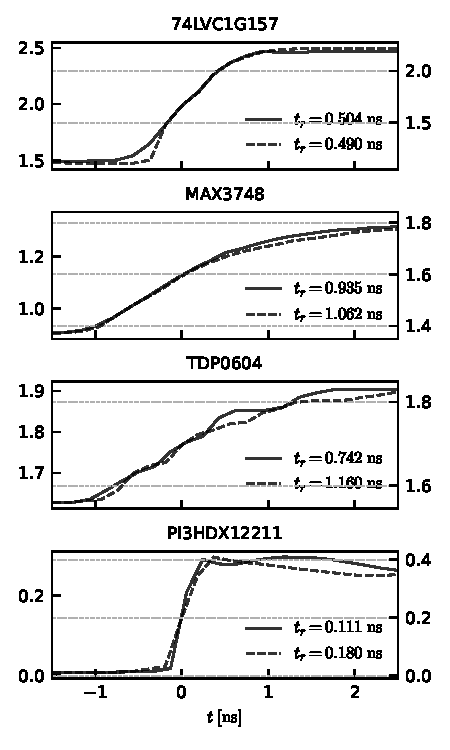
\includegraphics[width=\textwidth]{fig_edge_risetime.pdf}
    \end{center}
    \caption{The trailing edge of the stimulus pulse with no mesh connected measured by the board itself, using
    different amplifier ICs. Both positive and negative channels of the differential pair are shown individually.
    Vertical scale is in Volts at the sampling amplifier output.}
    \label{fig_edge_risetime}
\end{figure}

\begin{table}
    \begin{center}
        \begin{tabular}{r|cccc}
            \textbf{IC}
            &\texttt{74LVC1G157}
            &\texttt{MAX3748}
            &\texttt{TDP0604}
            &\texttt{PI3HDX12211}\\\hline
            \textbf{$t_r$}&
            \qty{497}{\pico\second}&
            \qty{998}{\pico\second}&
            \qty{951}{\pico\second}&
            \qty{145}{\pico\second}
        \end{tabular}
    \end{center}
    \caption{Single-ended stimulus edge rise times for different amplifier ICs. The single-ended rise times of both
    positive and negative half of the differential pair have been averaged.}
    \label{tab_edge_risetime}
\end{table}

\begin{figure}
    \begin{center}
        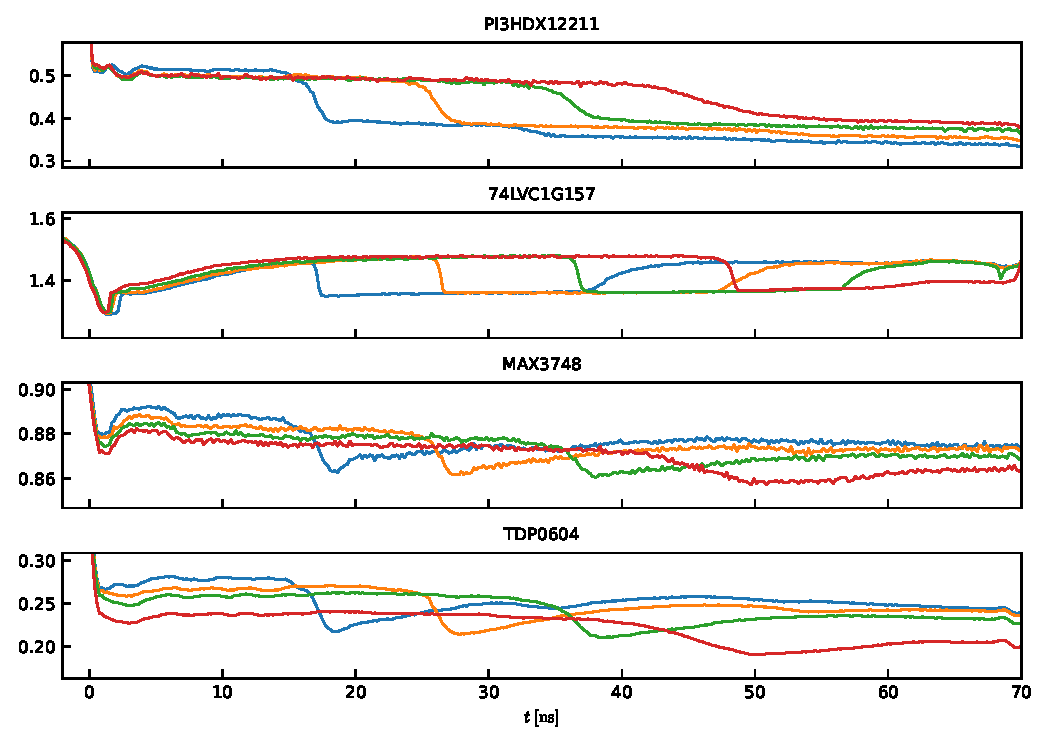
\includegraphics[width=\textwidth]{fig_mesh_length.pdf}
    \end{center}
    \caption{}
    \label{fig_mesh_length}
\end{figure}

\subsection{Tamper tests}

\begin{figure}
    \begin{center}
        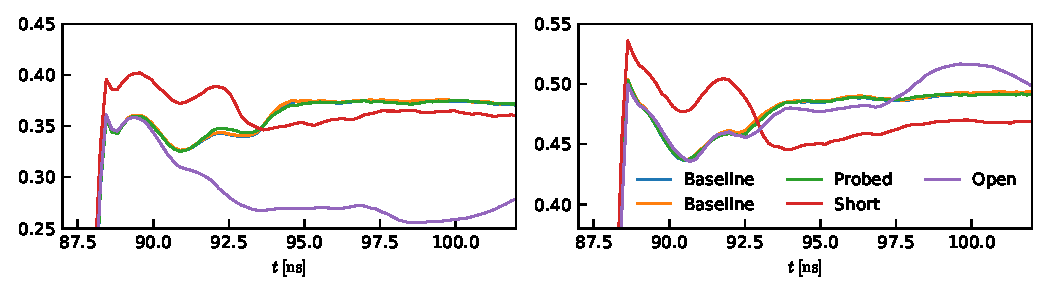
\includegraphics[width=\textwidth]{fig_manip_shape.pdf}
    \end{center}
    \caption{}
    \label{fig_manip_shape}
\end{figure}

\begin{figure}
    \begin{center}
        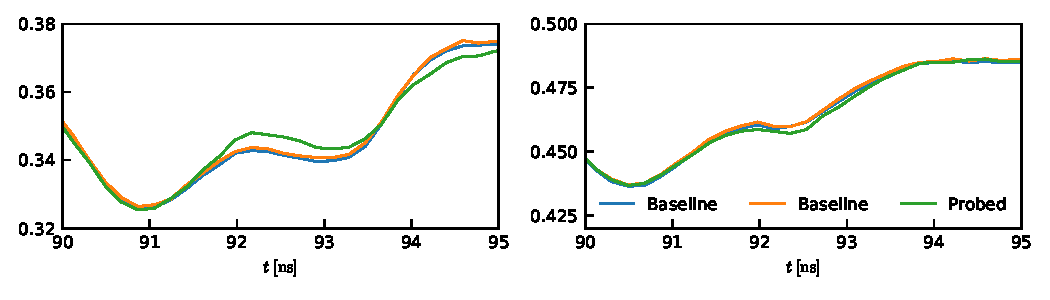
\includegraphics[width=\textwidth]{fig_probe_shape.pdf}
    \end{center}
    \caption{}
    \label{fig_probe_shape}
\end{figure}
% spectrum analyzer-measured reconstructed rise times for PI3HDX12211 (new measuremewnts!) ONET8501 and TDP0604
% Length measurements for all four different meshes
% One constructed mesh discontinuity example

\section{Conclusion}

In this paper, we presented a design for a low-cost frontend for the integrity monitoring security meshes in
applications such as HSMs based on the principles of sub-nanosecond Time-Domain Reflectometry. Our design
repurposes an inexpensive HDMI redriver IC to produce sharp edges for the TDR stimulus, and applies a microwave clip
line to form fast pulses for TDR sampling. Our design not only enables the monitoring of continuity and length of the
mesh's traces, but also allows monitoring the impedance at every point along the mesh. Our approach will not only detect
faults or manipulations that disturb the mesh without causing breaks, but it will also physically localize the point
where the fault occurs along the mesh. Compared to previous work, our approach provides an additional time dimension in
its characterization of a security mesh while simultaneously being less expensive, enabling more sophisticated tamper
detection algorithms.

\section*{Availability}
This is version \texttt{v0-draft-7-g4e03dc8-dirty
\unskip} of this paper, generated on \today.

The git repository with the LaTeX source for this paper, all hardware design files, and firmware and analysis source
code can be found at:

 \center{\url{https://git.jaseg.de/ihsm-sampling-mesh-monitor-hw.git}}

\FloatBarrier
\printbibliography[heading=bibintoc]
\end{document}
